\chapter{Supplementary Experiments}

\begin{figure}[htpb]
  \centering
  \captionof{figure}{Comparison of basic DQN network performance}
  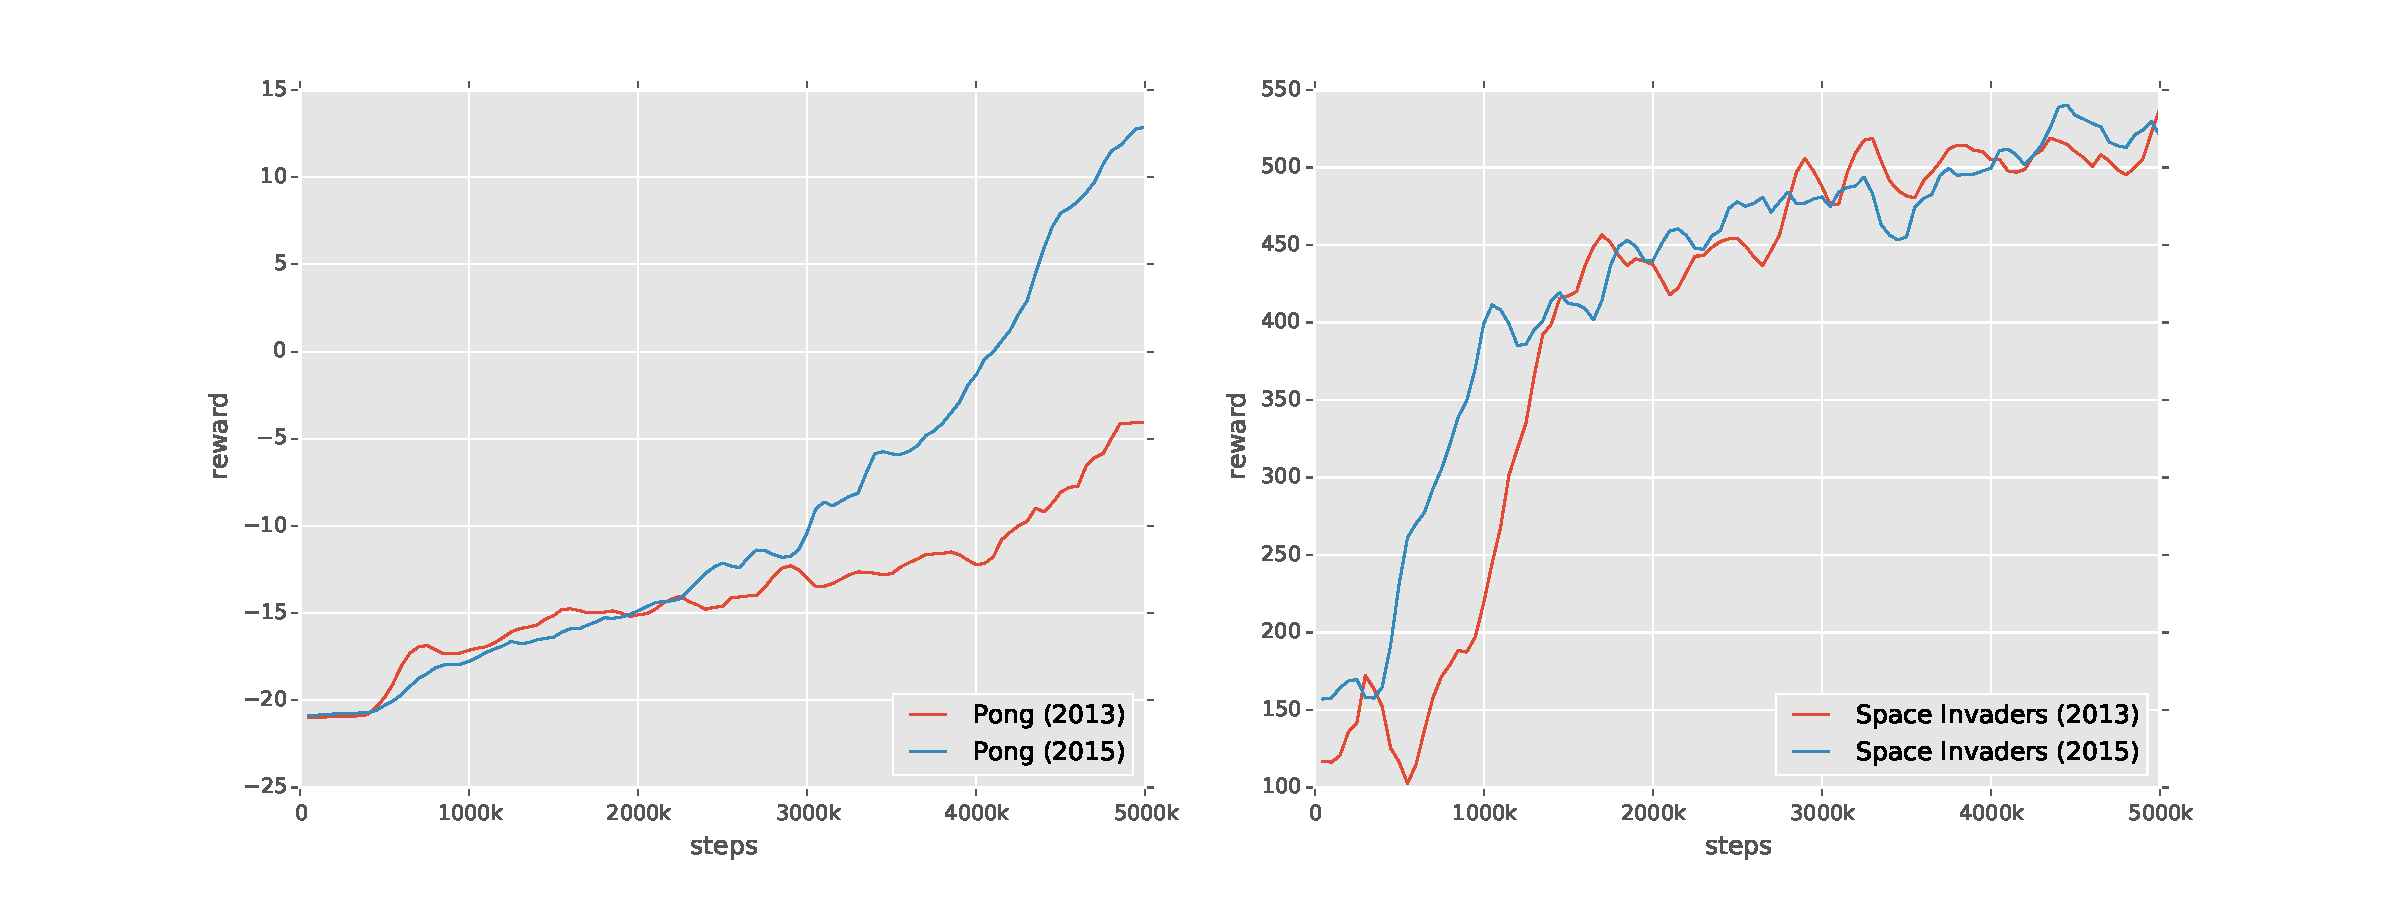
\includegraphics[width=1.0\linewidth]{nips_vs_nature_rewards.pdf}
  \raggedright
  \paragraph{}
    A comparison of learning curves for the two architectures described in
    \cite{Mnih2013} and \cite{Mnih2015}
    with network structure depicted in Figure \ref{fig:dqn_networks}
    and parameters in Table \ref{tab:boost}.

    Some games benefit more from increased network capacity than others.
  \label{fig:nips_vs_nature_rewards}
\end{figure}

\begin{figure}[htpb]
\end{figure}

\begin{figure}
  \vspace{-2cm}
 \begin{minipage}{1\textwidth}
  \centering
  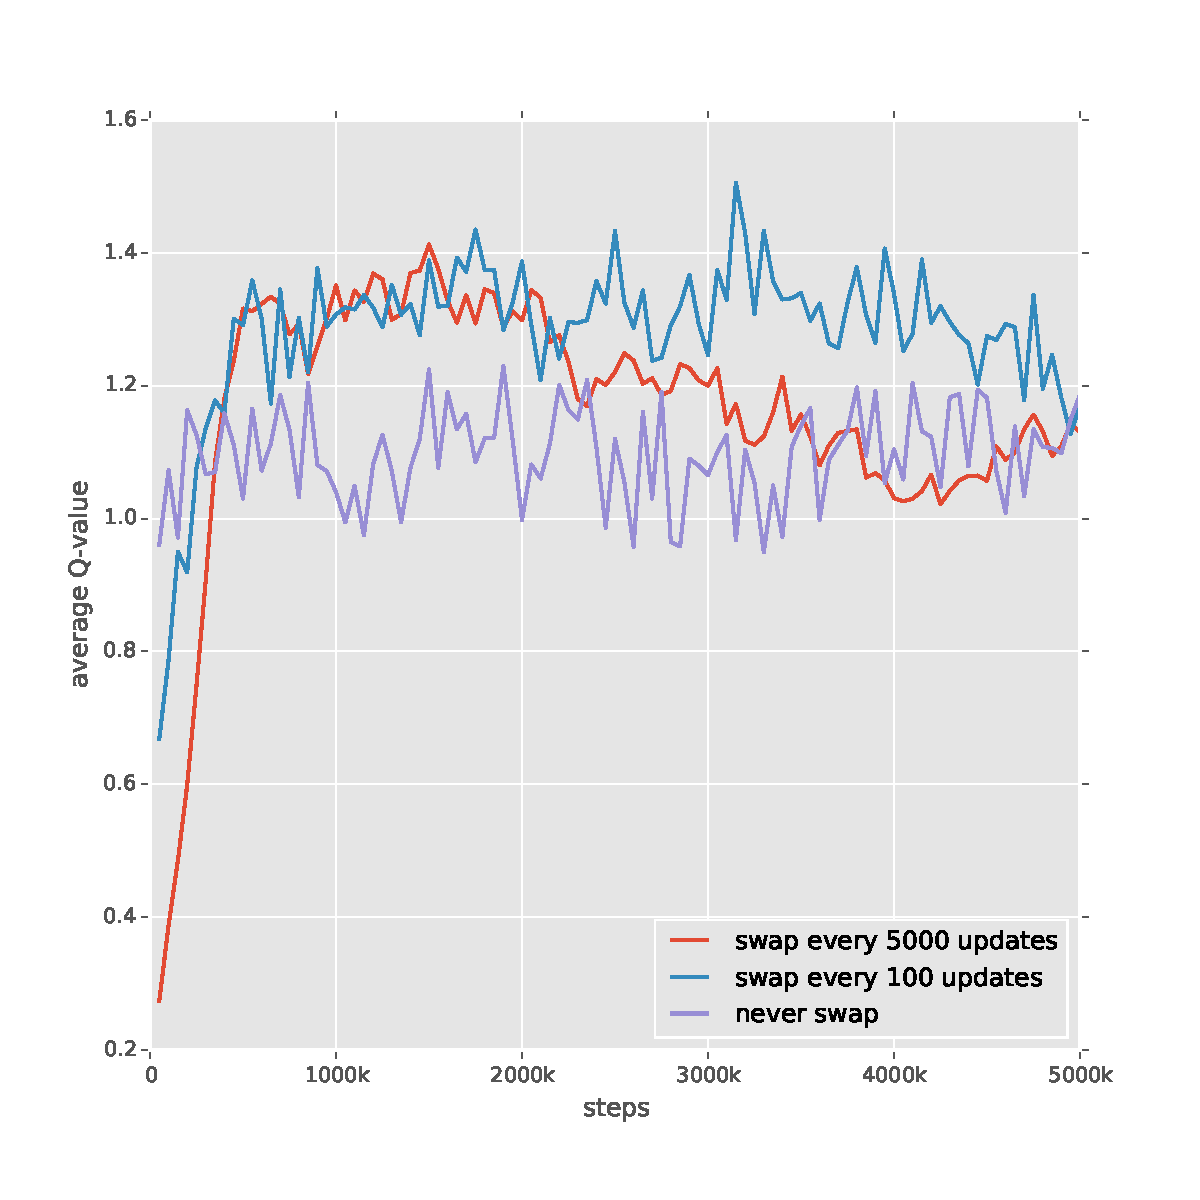
\includegraphics[width=0.6\linewidth]{freeze_qs.pdf}
  \caption[Target swap frequency comparison]{
    This graph depicts three runs of the game Space Invaders,
    each with a different interval for swapping
    the target Q-network,
    a measure that has been added to stabilize learning.

    The run that uses no separate target network
    does not really seem to learn any Q-values reliably
    while the network with the longest stable interval
    performs least noisily
    and actually seems to learn values.
  }
  \label{fig:freeze_qs}
 \end{minipage}
 \begin{minipage}{1\textwidth}
  \centering
  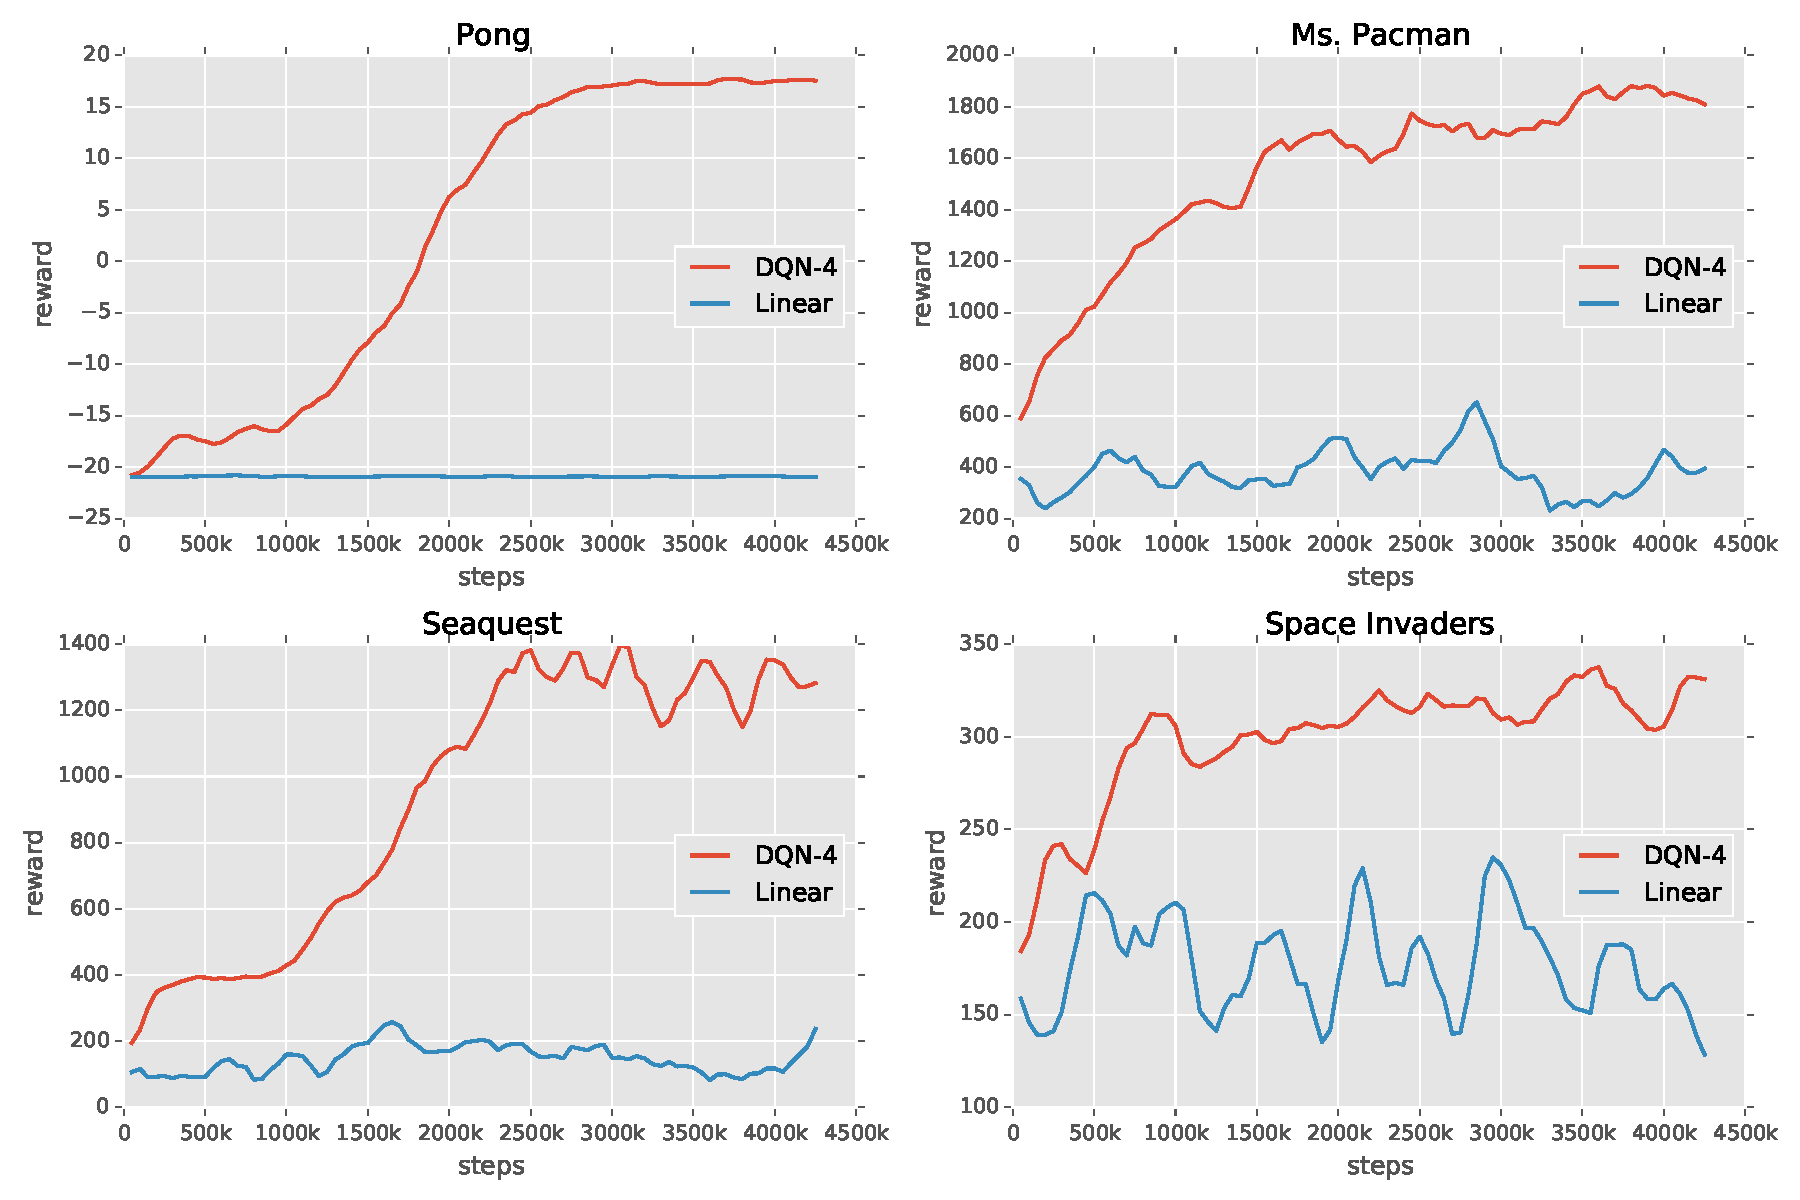
\includegraphics[width=1\linewidth]{dqn_vs_linear.pdf}
  \caption[Comparison of DQN versus linear mod]{
    Comparison of rewards over time of the DQN network
    versus a linear learner
    on 4 different games.
    Note that the linear results are not averaged,
    these are just from a single run.

    The linear model exists out of a single fully-connected layer.
  }
  \label{fig:dqn_vs_linear}
 \end{minipage}
\end{figure}
